\subsection{Limitations}
\label{sec:seq:limitations}

The main limitation for the sequential versions is the locality of the mesh used in the problem. Since this issue will be present in any shared memory implementation too, that discussion is left for \cref{sec:omp:limitations}.

\Cref{fig:roofline} shows the roofine for SeARCH Group 201 with the computational intensities of the SOA and AOS versions. Computational intensity is defined to be the ratio between all the instructions not related with memory accesses (loads and stores) and the number of bytes accessed in RAM.

The improvement from AOS to SOA can be explained only by the improvements in locality. Further testing, which results were omitted in this document, shown that the number of bytes accessed to RAM, number of computational instructions completed and the core functions execution time all decreased, achieving almost the same amount of computational instructions per second, while halving the number of accesses.

\begin{figure}
	\centering
	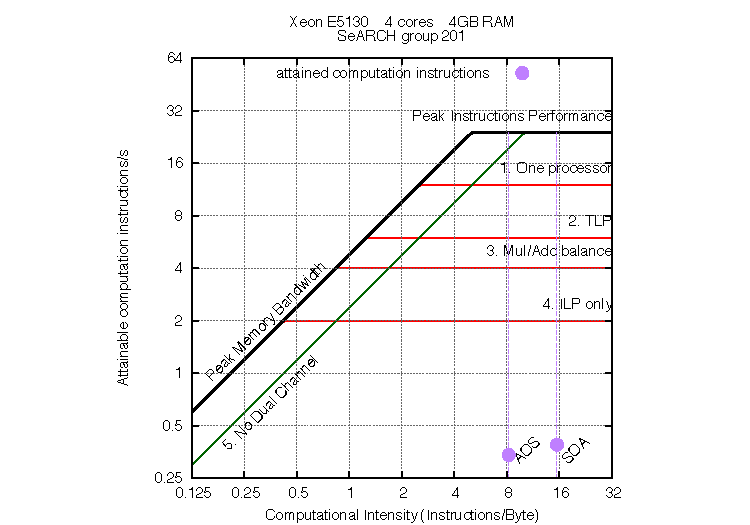
\includegraphics[width=\columnwidth]{images/roofline201m}
	\caption{Roofline for SeARCH Group 201, with the computational intensities of the AOS and SOA versions.}
	\label{fig:roofline201}
\end{figure}
